\subsection{Behaviour Tree evolved using an Evolutionary Algorithm}
Behaviour trees are trees of nodes (behaviours) which can either be basic (leaf), composite or decorator behaviours. A basic behaviour contains a single behaviour, such as "Flee" in the Ms. PacMan game. These basic behaviours generally serve a single purpose, which can be anything from evaluate how much danger the agent is in to attacking enemies. A behaviour tree is built around the use of these basic nodes in composite nodes. These composite nodes can be sequences or selectors. A sequence runs its child behaviours in order, failing if any of them fails. A selector does the same as a sequence, except it succeeds if any of its children succeed. Finally, decorators alters the output of its child node (such as inverting failed to success)\cite{simpsonBT}. In the implementation of the behaviour tree used for the controller covered in this paper, a \textit{PacManContext} object is used to keep track of game state values and behaviour parameters.

The most important components of evolutionary algorithms are the following six: \textit{representation}, \textit{evaluation function}, \textit{population}, \textit{parent selection mechanism}, \textit{variation operators}, and \textit{survivor selection mechanism}\cite{eiben2003introduction}. \textit{representation} is how the possible solutions in the original problem context (phenotypes) and their encodings (genotypes), individuals used in the evolutionary algorithm, are represented. The \textit{evaluation function} is used to determine the fitness of each phenotype. The \textit{population} contains the current generation of individuals. \textit{parent selection mechanism} is used to determine how many, and which, parents should be used to generate the next generation. The \textit{variation operators} determines the way and the amount that children differ from their parents in each generation. The \textit{survivor selection mechanism}

In this paper, an evolutionary algorithm is used to evolve to the parameters of the \textit{PacManContext} use by the behaviour tree. The \textit{PacManContext} is the phenotype from which a genotype, \textit{PMCGenotype}, that holds only the three parameters is constructed. 

\subsubsection{Algorithm Parameters}
The behaviour tree controller evolved for Ms. PacMan consists of three different parameters; the minimum distance to a ghost before PacMan begins fleeing, how far PacMan should look ahead while fleeing, and how close a ghost must be for PacMan to consider eating it once a power pill is active. The behaviour tree controller used in the competition used the following values: minimum\_distance= \textbf{8}, flee\_range = \textbf{36}, and eat\_distance = \textbf{19}.

\begin{figure}[htp]
\centerline{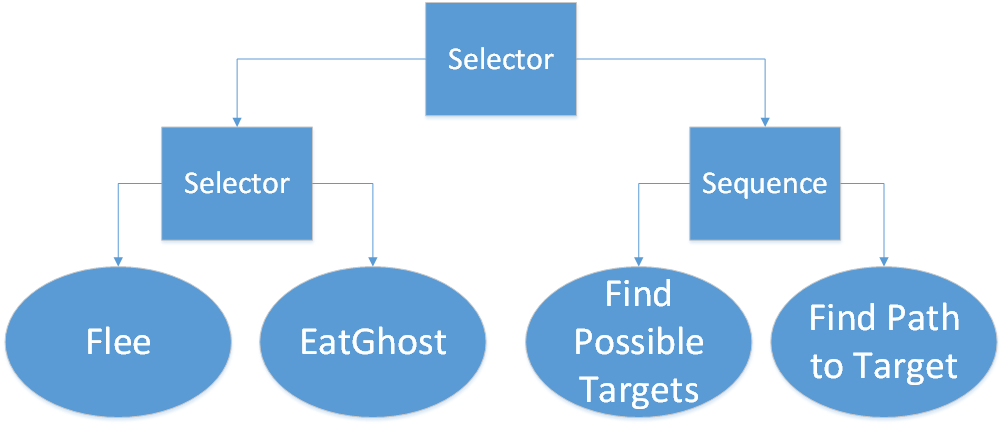
\includegraphics[width=1\columnwidth]{BehaviourTree}}
\caption{Structure of the behaviour tree used in the controller}
\label{figure-BT}
\end{figure}

Figure \ref{figure-BT} shows the chosen structure of the behaviour tree used by the evolved controller. No experimentation was done to the structure of the tree, except for early functionality tests. This was due to plenty of variation in average scores in just this structure and the different parameters for this specific behaviour tree.

Due to the non-deterministic nature of the Ms. PacMan game, the fitness value of an individual in the population was determined by taking the average of \textbf{1000} trials using the individual's decoded phenotype. Survivors were selected purely based on their fitness value. Evolution was done using only mutation and no recombination of parents. From experimentation, a population of \textbf{10} was kept of which \textbf{2} were selected as parents to produce \textbf{5} children each per generation. A generation limit of \textbf{200} was used due to only minuscule changes after around 190 generations. The variables of each of the individuals in the initial generation were initialised randomly between 0 and a maximum value: min\_distance\_max\_value = \textbf{40}, flee\_distance\_max\_value = \textbf{200}, and eat\_distance\_max\_value = \textbf{400}. Each variable of the individuals were mutated by \textbf{10\%} of their maximum value.

The solution with the highest fitness value after the 200 generations used the following parameters: minimum\_distance = \textbf{5}, flee\_range = \textbf{36}, and eat\_distance = \textbf{155}.